\documentclass{classe-tex3R-2-1}

\usepackage{style-tex3R-2-1}
\usepackage{lipsum}


\usetikzlibrary{arrows.meta,
calc, chains, % added
positioning, % added
shapes}
\makeatletter
\tikzset{FlowChart/.style={% enable to be used also at other flowcharts
suspend join/.code={\def\tikz@after@path{}},
startstop/.style = {rectangle, rounded corners, draw, fill=red!30,
minimum width=3cm, minimum height=1cm,
on chain, join=by line},
block/.style = {rectangle, draw, %fill=blue!30,
text width=4cm, minimum height=1cm, align=center,
on chain, join=by line},
decision/.style = {diamond, aspect=1.3, draw, fill=gray!30,
text width=3cm, minimum height=1cm, align=center,
on chain, join=by line},
line/.style = {thick,-Triangle}
} }
\makeatother



\begin{luacode}
PARAMETRES = {}

format = 'fiche'

PARAMETRES.format = 'diapo'
PARAMETRES.type = 'TD'
PARAMETRES.enonce = true
PARAMETRES.correction = true
PARAMETRES.theme = true
PARAMETRES.cache = true
PARAMETRES.header = true
PARAMETRES.print = false
PARAMETRES.visible = false
PARAMETRES.difficulte = true
PARAMETRES.competence = true
PARAMETRES.source = true
PARAMETRES.theme = true
PARAMETRES.visible = false


-- PARAMETRES.taille = '50pt'
-- PARAMETRES
\end{luacode}

\parametrage

\niveau{5}
\chapitre{4}{Théorème de Thalès}


\begin{document}

test

\includegraphics[]{example-image-a}


\includegraphics[]{demenagement.eps}

\begin{scratch*}[print]
\blockmove{tourner de \turnleft{} de \ovalnum{45} degrés}
\blocklook{penser à \ovalnum{Hmm..} pendant \ovalnum{2} secondes}
\blocklook{penser à \ovalsensing{réponse}}
\blockmove{aller à x: \ovaloperator{\ovalmove{ abscisse x} + \ovalnum{1}} y: \ovalmove{ordonnée y}}
\blocksound{jouer le son \ovalsound*{Meow}}
\blockcontrol{créer un clone de \ovalcontrol*{moi même}}
\end{scratch*}

\DecompositionDecimale{12.395}




\Tables{}



\Tableau[CarreA,Colonnes,Fleches]{}

\Thales[Figurecroisee,ChoixCalcul=1,Droites]{ABCMN}{35}{90}{7}{AB}{AC}{12}


\begin{center}
\Propor[Stretch=1.25,%
Math,%
GrandeurA=Hauteur $h$ (\Lg{}),%
GrandeurB=\begin{tabular}{c}Volume (en \Vol{}) d'un cylindre\\ de rayon \Lg{5} et
de hauteur $h$\end{tabular},%
Largeur=0.75cm]{2/$50\pi$,3/$75\pi$,5/}
\end{center}
\FlecheLineaireH{1}{2}{3}{$+$}
\FlecheLineaireB{1}{2}{3}{$+$}
\FlechePCB{3}{2}

\tikzstyle{FlechePropor}=[-{Stealth[
length=3mm, width=2mm]}]
\begin{center}
\Propor[Stretch=2]{1/2.5,2/5,5/12.5}
\end{center}
\FlechesPH{1}{2}{$\times2$}
\FlechesPB{1}{3}{$\times5$}
\FlechesPD{1}{2}{$\times\num{2,5}$}
\FlechesPG{2}{1}{$\div\num{2,5}$}

\begin{pspicture}(-1,-2)(10,5)

\psgrid[griddots=5, subgriddiv=0, gridlabels=1pt](-1,-2)(10,5)
% Croquis carte
\psline(0,0)(5,0)(5,4)(0,4)(0,0)


% croquis capteur
\psline(7,1)(9,1)(9,4)(7,4)(7,1)

\pscircle(0.5,0.8){0.2}
\pscircle(1.5,0.8){0.2}
\pscircle(2.5,0.8){0.2}
\pscircle(3.5,0.8){0.2}
\pscircle(4.5,0.8){0.2}

\pscircle*(0.5,00){0.1}
\pscircle*(1.5,00){0.1}
\pscircle*(2.5,00){0.1}
\pscircle*(3.5,00){0.1}
\pscircle*(4.5,00){0.1}

\rput[b](0.5,0.2){0}
\rput[b](1.5,0.2){1}
\rput[b](2.5,0.2){2}
\rput[b](3.5,0.2){3V}
\rput[b](4.5,0.2){GND}

\psframe*(7.3,0)(7.4,1)
\rput[b]{90}(7.5,1.6){Signal}

\psframe*(7.95,0)(8.05,1)
\rput[b]{90}(8.15,1.4){3V}

\psframe*(8.6,0)(8.7,1)
\rput[b]{90}(8.75,1.5){GND}

\rput[t](2.5,4.5){Carte micro:bit}

\rput[b](8,4.5){Capteur:\visible{ \dots}{Vibrations}}
\rput[t](8,4.4){Ref: \visible{\dots}{ KY-0.31}}

\ifcorrection
\psline[linearc=0.2,linewidth=0.1,linecolor=Brown](4.5,0)(4.5,-0.5)(8.65,-0.5)(8.65,0)
\psline[linearc=0.2,linewidth=0.1,linecolor=Green](0.5,0)(0.5,-1)(7.35,-1)(7.35,0)
\psline[linearc=0.2,linewidth=0.1,linecolor=Red](3.5,0)(3.5,-1.5)(8,-1.5)(8,0)
\fi

\end{pspicture}

\adjustbox{valign=t}{\begin{minipage}{0.48\linewidth}%
		\begin{tikzpicture}
			\tkzDefPoints{0/4/A,0/0/B,3/0/C,3/4/D,5/0/E,0/-1/Y,5/-1/Z}
			\tkzLabelPoints[above](A,D)
			\tkzLabelPoints[below](B,C,E)
			\tkzDrawSegments(A,B B,C C,E E,D D,A)
			\tkzDrawSegments[style=dashed](D,C)
			\tkzMarkRightAngle(D,A,B)
			\tkzMarkRightAngle(A,B,C)
			\tkzMarkRightAngle(B,C,D)
			\tkzMarkRightAngle(C,D,A)
			\tkzDrawSegment[{Latex[scale=1.5]}-{Latex[scale=1.5]}](Y,Z)
			\tkzLabelSegment[pos=0.5,below](Y,Z){$\np[cm]{7.5}$}
			\tkzLabelSegment[pos=0.5,left](A,B){$\np[cm]{5.6}$}
			\tkzLabelSegment[pos=0.5,above](A,D){$\np[cm]{3.2}$}
		\end{tikzpicture}
\end{minipage}}\hfill%
\adjustbox{valign=t}{\begin{minipage}{0.48\linewidth}%
		\begin{tikzpicture}
		\tkzDefPoints{0/2/A,4/2/B,4/0/C,0/0/D,0/1/E,4/1/F,5.5/0/Y,5.5/2/Z}
		\tkzLabelPoints[above](A,B)
		\tkzLabelPoints[below](C,D)
		\tkzDrawSegments(A,B C,D)
		\tkzDrawSegments[style=dashed](B,C D,A)
		\tkzDrawArc(E,A)(D)
		\tkzDrawArc(F,C)(B)
		\tkzMarkRightAngle(D,A,B)
		\tkzMarkRightAngle(A,B,C)
		\tkzMarkRightAngle(B,C,D)
		\tkzMarkRightAngle(C,D,A)
		\tkzLabelSegment[pos=0.5,below](D,C){$\np[cm]{8.4}$}
		\tkzDrawSegment[{Latex[scale=1.5]}-{Latex[scale=1.5]}](Y,Z)
		\tkzLabelSegment[pos=0.5,right](Y,Z){$\np[cm]{2.1}$}
	\end{tikzpicture}

\vspace{0.2cm}

\begin{tikzpicture}
	\tkzDefPoints{0/0/A,4/0/B,1/1/D,5/1/C,5/2.41/E,6/0/Y,6/1/Z}
	\tkzDrawSegments(A,B B,C C,E E,D D,A)
	\tkzDrawSegments[style=dashed](D,Z B,Y)
	\tkzLabelPoints[above](E)
	\tkzLabelPoints[below](A,B)
	\tkzLabelPoints[right, below](C)
	\tkzLabelPoints[left](D)
	\tkzMarkSegments[pos=0.5,mark=s||](A,B D,C)
	\tkzMarkSegments[pos=0.5,mark=s|](A,D B,C C,E)
	\tkzMarkRightAngle(D,C,E)
	\tkzLabelSegment[pos=0.5,below=0.2](A,B){$\np[cm]{4.7}$}
		\tkzLabelSegment[pos=0.5,right](E,C){$\np[cm]{1.2}$}
	\tkzDrawSegment[{Latex[scale=1.5]}-{Latex[scale=1.5]}](Y,Z)
	\tkzLabelSegment[pos=0.5,right](Y,Z){$\np[cm]{0.8}$}
\end{tikzpicture}
\end{minipage}}%

\newpage




\visible{Ce texte est visible quand visible=true}{Celui ci quand visible = false}

\begin{visible*}
Ceci est visible quand visible = true
\end{visible*}













\begin{visible*}[true]
Ceci est visible quand visible = true
\end{visible*}

\begin{visible*}[false]
Ceci est visible quand visible = false
\end{visible*}


\newpage

\begin{center}
\scalebox{0.9}{ 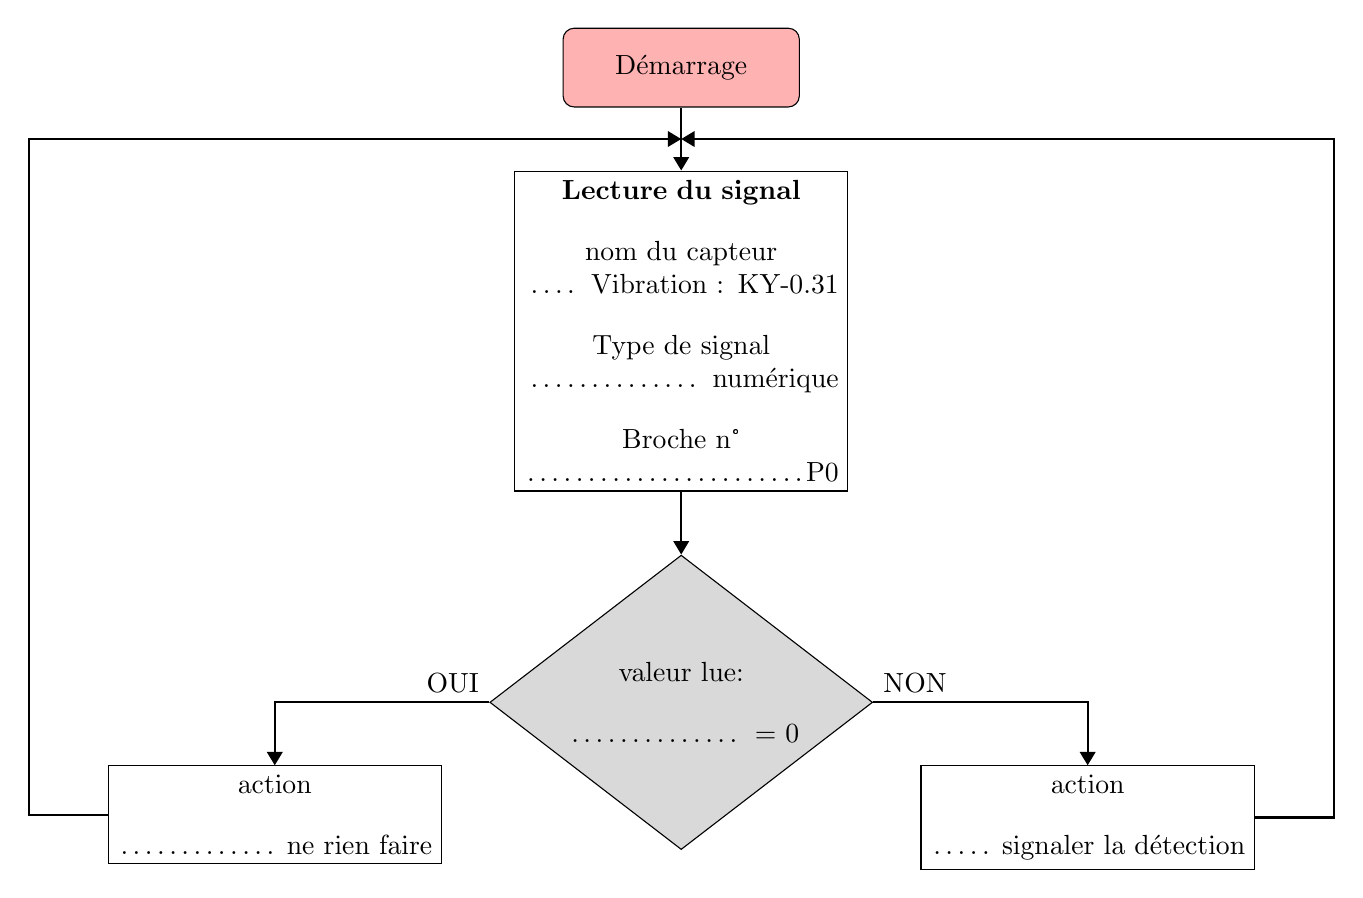
\begin{tikzpicture}[FlowChart, auto,
node distance = 8mm and 6mm,
start chain = going below
]
% Place nodes
\node (init) [startstop]{Démarrage};
\node (tag1) [block] {\textbf{Lecture du signal} \par\vspace{1em}nom du capteur \par \visible{ \dotfill}{ Vibration : KY-0.31} \par \vspace{1em} Type de signal \par \visible{ \dotfill}{ numérique}\par \vspace{1em} Broche n° \par\visible{ \dotfill}{P0}};

\node (tag2) [decision]{valeur lue:\par\vspace{1em}\visible{ \dotfill}{ = 0}};
\node (tag3a) [block,suspend join, below left=of tag2.west] {action \par \vspace{1em}\visible{ \dotfill}{ ne rien faire}};
\node (tag3b) [block, suspend join, below right=of tag2.east] {action \par \vspace{1em}\visible{ \dotfill}{ signaler la détection}};


\draw[line] (tag2.west) node[above left] {OUI} -|(tag3a);
\draw[line] (tag2.east) node[above right] {NON} -| (tag3b);

\draw[line] (tag3a.west) node[above left]{}-- ++ (-1,0) |- ($(init.south)!0.5!(tag1.north)$);
\draw[line] (tag3b.east) node[above right]{}-- ++ (1,0) |- ($(init.south)!0.5!(tag1.north)$);

\end{tikzpicture}}
\end{center}

% \ifdiapo \textcolor{green}{diapo}\par \else \hfill \textcolor{red}{no} \textcolor{red}{diapo}\par \fi
% \iffiche \textcolor{green}{fiche}\par \else \hfill \textcolor{red}{no} \textcolor{red}{fiche}\par \fi
% \ifheader \textcolor{green}{header}\par \else \hfill \textcolor{red}{no} \textcolor{red}{header}\par \fi

% % \bigskip

% \ifenonce \textcolor{green}{enonce}\par \else \hfill \textcolor{red}{no} \textcolor{red}{enonce}\par \fi
% \ifcorrection \textcolor{green}{correction}\par \else \hfill \textcolor{red}{no} \textcolor{red}{correction}\par \fi

% % \bigskip


% \iftheme \textcolor{green}{theme}\par \else \hfill \textcolor{red}{no} \textcolor{red}{theme}\par \fi
% \ifcache \textcolor{green}{cache}\par \else \hfill \textcolor{red}{no} \textcolor{red}{cache}\par \fi
% \ifdifficulte \textcolor{green}{difficulte}\par \else \hfill \textcolor{red}{no} \textcolor{red}{difficulte}\par \fi
% \ifcompetence \textcolor{green}{competence}\par \else \hfill \textcolor{red}{no} \textcolor{red}{competence}\par \fi
% \ifsource \textcolor{green}{source}\par \else \hfill \textcolor{red}{no} \textcolor{red}{source}\par \fi


% \bigskip

% \ifactivite \textcolor{green}{activite}\par \else \hfill \textcolor{red}{no} \textcolor{red}{activite}\par \fi
% \ifbasique \textcolor{green}{basique}\par \else \hfill \textcolor{red}{no} \textcolor{red}{basique}\par \fi
% \ifcorrige \textcolor{green}{corrige}\par \else \hfill \textcolor{red}{no} \textcolor{red}{corrige}\par \fi
% \ifcours \textcolor{green}{cours}\par \else \hfill \textcolor{red}{no} \textcolor{red}{cours}\par \fi
% \ifTD \textcolor{green}{TD}\par \else \hfill \textcolor{red}{no} \textcolor{red}{TD}\par \fi
% \ifflash \textcolor{green}{flash}\par \else \hfill \textcolor{red}{no} \textcolor{red}{flash}\par \fi
% \ifDM \textcolor{green}{DM}\par \else \hfill \textcolor{red}{no} \textcolor{red}{DM}\par \fi
% \ifDS \textcolor{green}{DS}\par \else \hfill \textcolor{red}{no} \textcolor{red}{DS}\par \fi
% \ifinterro \textcolor{green}{interro}\par \else \hfill \textcolor{red}{no} \textcolor{red}{interro}\par \fi

% \bigskip

% \ifprint \textcolor{green}{print}\par \else \hfill \textcolor{red}{no} \textcolor{red}{print}\par \fi

%\ifFirstCompile \textcolor{green}{FirstCompile}\par \else \hfill \textcolor{red}{no} \textcolor{red}{FirstCompile}\par \fi

% \bigskip

% 23 \iflignes \textcolor{green}{lignes}\par \else \hfill \textcolor{red}{no} \textcolor{red}{lignes}\par \fi
% / \ifseyes \textcolor{green}{seyes}\par \else \hfill \textcolor{red}{no} \textcolor{red}{seyes}\par \fi
% 101 \ifsurligne \textcolor{green}{surligne}\par \else \hfill \textcolor{red}{no} \textcolor{red}{surligne}\par \fi
% 83 \ifcarreaux \textcolor{green}{carreaux}\par \else \hfill \textcolor{red}{no} \textcolor{red}{carreaux}\par \fi
% 73 \iflignesetoile \textcolor{green}{lignesetoile}\par \else \hfill \textcolor{red}{no} \textcolor{red}{lignesetoile}\par \fi
% / \ifseyesetoile \textcolor{green}{seyesetoile}\par \else \hfill \textcolor{red}{no} \textcolor{red}{seyesetoile}\par \fi
% 89 \ifcarreauxetoile \textcolor{green}{carreauxetoile}\par \else \hfill \textcolor{red}{no} \textcolor{red}{carreauxetoile}\par \fi

% \bigskip

% ? \ifaffichagetitre \textcolor{green}{affichagetitre}\par \else \hfill \textcolor{red}{no} \textcolor{red}{affichagetitre}\par \fi
% / \ifmegadoctoc \textcolor{green}{megadoctoc}\par \else \hfill \textcolor{red}{no} \textcolor{red}{megadoctoc}\par \fi
% / \ifmegadoc \textcolor{green}{megadoc}\par \else \hfill \textcolor{red}{no} \textcolor{red}{megadoc}\par \fi

% \newpage test

\end{document}